

The software we'll be building in this chapter isn't meant to be extremely complex – we'll create a simple calculator that adds two numbers together (Figure 12.1). It will be released as a console application with a text user interface and a library to perform mathematical operations, which can potentially be used in another project. While there isn't much use for such a project in real life, as C++ offers plenty of support for calculations in its standard library, its banality will be perfect to explore how all techniques discussed in this book work together in practice:

\begin{center}
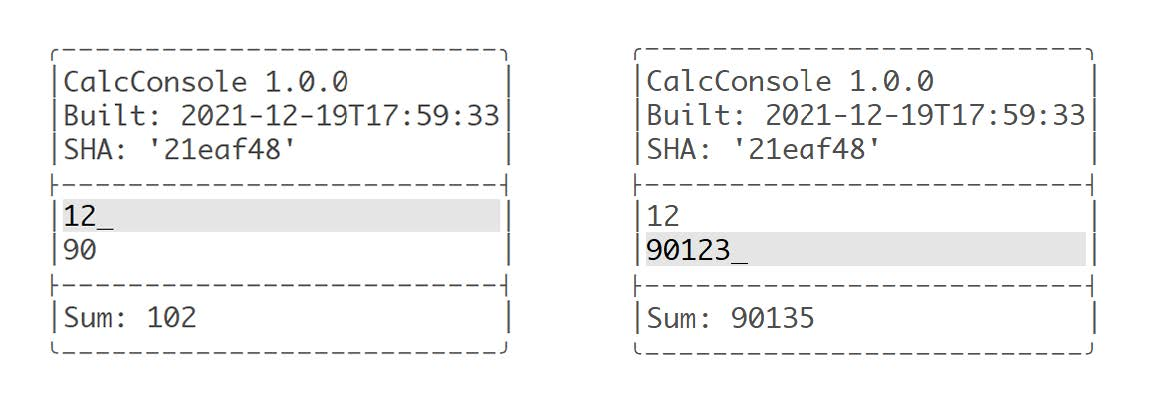
\includegraphics[width=0.8\textwidth]{content/3/chapter12/images/1.jpg}\\
Figure 12.1 – The two states of a console calculator's user interface
\end{center}

Usually, projects either produce a user-facing executable or a library for developers. Projects that do both are a bit rarer but not totally uncommon – some applications offer standalone SDKs or libraries supporting the creation of plugins. Another case may be a library that offers examples of its usage. The project we'll build in this chapter somewhat fits into the last category.

We will start planning by reviewing the list of chapters, recalling their content, and selecting the techniques and tools described therein that we will use to build our computing application: 

Chapter 1, First Steps with CMake: 

The first chapter gave us basic information on CMake – how to install it and use its command line to build prepared projects. Information on project files provided here will be key: the responsibilities of different files, conventionally used names, and some quirks. In this chapter, we also discussed preset files for generators, but we'll skip these in this project.

Chapter 2, The CMake Language: 

Here, we introduced tools necessary to write correct listfiles and scripts. We shared fundamental information on code: comments, command invocations, and arguments. We also thoroughly explained variables, lists, and control structures and presented a few very useful commands. This knowledge will be applied throughout the project.

Chapter 3, Setting Up Your First CMake Project:

Topics covered in the third chapter will have a critical impact on the project:

\begin{itemize}
\item 
Specifying a minimal CMake version decides which CMake policies will apply; naming, versioning, and configuring a project's language affects the basic behavior of the build.

\item 
Insights into project partitioning and structuring that shape the layout of directories and files.

\item 
System discovery variables to help us decide how to handle different environments, specifically for this project – for example, do we need to run ldconfig?

\item 
Toolchain configuration allows the requirement of a particular version of C++ and a standard supported by the compiler.
\end{itemize}

This chapter also tells us that it's often a good idea to disable in-source builds, so we'll do that.

Chapter 4, Working with Targets: 

Here, we highlighted how every modern CMake project makes extensive use of targets. Ours will too, for the following reasons:

\begin{itemize}
\item 
Defining a few libraries and executables (both for test and production) will keep the project organized and DRY.

\item 
Target properties and transitive usage requirements (propagated properties) keep configuration close to target definitions.

\item 
Generator expressions are going to appear throughout the solution, but we'll keep them as simple as possible.
\end{itemize}

In this project, we'll use custom commands to generate files for Valgrind and coverage reports, and we'll use target hooks (PRE\_BUILD) to clean the .gcda files produced by coverage instrumentation.

Chapter 5, Compiling C++ Sources with CMake: 

There's no C++ project without compilation. The basics are quite simple, but CMake allows us to tweak this process in so many ways: extend the sources of a target, configure the optimizer, and provide debugging information. For this project, the default compilation flags will do just fine, but we'll go ahead and play a bit with the preprocessor:

\begin{itemize}
\item 
We'll store build metadata (the project version, build time, and the Git commit SHA) in the compiled executable and show it to the user.
	
\item 
We'll enable the precompilation of headers. It's not really a necessity in such a small project, but it will help us practice this concept.
\end{itemize}

Unity builds won't be necessary – the project won't be big enough to make adding them worthwhile.

Chapter 6, Linking with CMake:

The sixth chapter provides us with general information on linking (useful in any project), most of which comes in handy by default. But since this project also provides a library, we'll explicitly refer to some building instructions on the following:

\begin{itemize}
\item 
Static libraries for testing and development

\item 
Shared libraries for release
\end{itemize}

This chapter outlines how to separate main() for testing, which we'll do as well.

Chapter 7, Managing Dependencies with CMake:

To make the project more interesting, we'll bring an external dependency: a text UI library. We described a few dependency management methods in this chapter. Picking the right one isn't too difficult: the FetchContent utility module is usually recommended and most convenient (unless we are solving a specific corner case described in the chapter).

Chapter 8, Testing Frameworks:

Proper automated tests are imperative to assure that quality of our solution doesn't degrade over time. We'll add the support for CTest and properly structure our project for testing (we'll apply the main() separation mentioned earlier).

Also, in this chapter, we discussed two testing frameworks: Catch2 and GTest with gMock; for this project, we'll use the latter. To get clear information on our coverage, we'll generate HTML reports with LCOV

Chapter 9, Program Analysis Tools:

To perform static analysis, we can choose from a variety of tools: Clang-Tidy, Cpplint, Cppcheck, include-what-you-use, and link what you use. In this case, we'll go with Cppcheck , as Clang-Tidy doesn't work very well with precompiled headers built with GCC. The dynamic analysis will be done with Valgrind's Memcheck tool, and we'll use the Memcheck-cover wrapper to generate HTML reports. Our source will be also automatically formatted during the build with ClangFormat.

Chapter 10, Generating Documentation:

Since we'll be providing a library as part of this project, it's key to provide at least some documentation to go with it. As we already know, CMake allows us to automate the generation of it with Doxygen. We'll do that in a refreshed design by adding the doxygenawesome-css look to it.

Chapter 11, Installing and Packaging:

Finally, we'll configure the installation and packaging of our solution. We'll prepare files to form the package as described, along with target definitions. We'll install that and the artifacts from build targets to appropriate directories by including the GNUInstallDirs module. We will additionally configure a few components to modularize the solution and prepare it for use with CPack.

Professional projects also come with a few text files: README, LICENSE, INSTALL, and so on. We'll touch on this briefly at the end.

\begin{tcolorbox}[colback=blue!5!white,colframe=blue!75!black,title=Note]
To make things simpler, we won't implement logic that checks whether all the required utilities and dependencies are available. We'll rely on CMake here to show its diagnostics and tell users what's missing. If projects that you publish after reading this book get significant traction, you might want to consider adding these mechanisms to improve the user experience.
\end{tcolorbox}

Having formed a clear plan, let's discuss how to actually structure the project, both in terms of logical targets and directory structure.
















